%%%%%%%%%%%%%%%%%%%%%%%%%%%%%%%%%%%%%%%%%
% Masters/Doctoral Thesis
%
% %%%%% IMPORTANT %%%%%
% 1) Edit Front/vars.tex
% 2) Compile Front/main.tex
% 3) Edit vars.tex
% 4) Edit precontent.tex
%
% BEFORE ANYTHING ELSE
% You can also set some interesting stuff in the preamble.tex file
% If you know what you're doing.
%%%%%%%%%%%%%%%%%%%%%%%%%%%%%%%%%%%%%%%%%

% The default font size and two-sided printing
% For a one-sided printing change the flag "twoside" to "oneside"
\documentclass[11pt, oneside, table,xcdraw]{Thesis}


%-------------------------------------------------------------------------
%   PREAMBLE AND SETTINGS
%-------------------------------------------------------------------------
% Add the preamble. You can change various settings in here
%-------------------------------------------------------------------------
%	PACKAGES AND OTHER DOCUMENT CONFIGURATIONS
%-------------------------------------------------------------------------

% Include pdf pages in the document
% Necessary to include the front pages (cover and etc.)
\usepackage{pdfpages}

% For the cover page
%\usepackage{tikz}

% Fix top page geometry on long titles
\setlength{\headheight}{14pt}  %Try fix error

% Language hyphenation and typographical rules
\usepackage[portuguese,english]{babel}
%Custom hyphenization
\hyphenation{Py-thon}
\hyphenation{Ju-py-ter}
\hyphenation{Ma-the-ma-ti-ca}

% Inline quotes
% added for \begin{displayquote}
\usepackage[autostyle]{csquotes}

% Bibliography setup
% Use the natbib reference package - read up on this to edit the reference
% style; if you want text (e.g. Smith et al., 2012) for the in-text references
% (instead of numbers), remove 'numbers'
\usepackage[square, numbers, comma, sort&compress]{natbib}
\bibliographystyle{IEEEtranN}  % I actually quite like this one
% \bibliographystyle{apsrev4-1-etal} % With emphasized titles. ORIGINAL
% Prevent that the first citation is in the ToC
\usepackage{notoccite}
\setlocalecaption{english}{bib}{References}


% Interesting float placements (like 'H') and custom float types
\usepackage{float}
% Text wrapped around pictures
% https://pt.sharelatex.com/learn/Wrapping_text_around_figures
\usepackage{wrapfig}
% Force float barriers, use as \FloatBarrier
\usepackage[section]{placeins}
% Place floats *above* footnotes
\usepackage[bottom, perpage, symbol]{footmisc}
% Set default float placement
\makeatletter
\renewcommand{\fps@figure}{tbph}
\renewcommand{\fps@table}{tbph}
\makeatother

% Pretty colours
\usepackage{xcolor}
% \usepackage{color} % Deprecated by xcolor

% SVGs with Inkscape and PDF+LaTeX
% https://tex.stackexchange.com/questions/473994/svg-and-inkscape
\usepackage[inkscapearea=page]{svg}
% Specifies the directory where vector are stored
\svgpath{{Svgs/}}

% Graphics stuff
\usepackage{graphicx}  % invoked by svg
% Specifies the directory where pictures are stored
\graphicspath{{Figures/}}

% For sub-figures and stuff
\usepackage{caption}
\usepackage{subcaption}

% Math stuff
\usepackage{amsmath} % Interesting environments
\usepackage{amssymb} % Interesting symbols
\usepackage{commath} % Interesting macros
\usepackage{braket} % Dirac bra-ket and set notations
\usepackage{mathpazo} % Math font (palatino for Computer Modern on math)
\usepackage{mathtools} % Mathematical tools to use with amsmath
\setstretch{1.5}
% Math alphabet
\DeclareMathAlphabet{\pazocal}{OMS}{zplm}{m}{n}
\newcommand{\Sa}{\pazocal{S}}
\newcommand{\Ua}{\pazocal{U}}
\newcommand{\Ha}{\pazocal{H}}
\newcommand{\Fa}{\pazocal{F}}
\newcommand{\Ia}{\pazocal{I}}
\newcommand{\Ea}{\pazocal{E}}
\newcommand{\ja}{\pazocal{J}}
%Custom math operators
\DeclareMathOperator*{\meshgrid}{meshgrid}
% Floor and ceiling of numbers
\DeclarePairedDelimiter\ceil{\lceil}{\rceil}
\DeclarePairedDelimiter\floor{\lfloor}{\rfloor}
% Notation variables
\newcommand{\dd}{\mathrm{d}}

% Units and numbers in text
\usepackage{siunitx}
\DeclareSIUnit\baud{Bd} % Baud

% Reimplementation of and extensions to LaTeX verbatim
\usepackage{verbatim} %added for \begin{comment}

% Fancy chapter start quotes
\usepackage{epigraph, varwidth}
% Overload epigraph command
\renewcommand{\epigraphsize}{\small}
\setlength{\epigraphwidth}{0.90\textwidth}
\renewcommand{\textflush}{flushright}
\renewcommand{\sourceflush}{flushright}
% A useful addition
\newcommand{\epitextfont}{\itshape}
\newcommand{\episourcefont}{\scshape}
\makeatletter
\newsavebox{\epi@textbox}
\newsavebox{\epi@sourcebox}
\newlength\epi@finalwidth
\renewcommand{\epigraph}[2]{%
  \vspace{\beforeepigraphskip}
  {\epigraphsize\begin{\epigraphflush}
   \epi@finalwidth=\z@
   \sbox\epi@textbox{%
     \varwidth{\epigraphwidth}
     \begin{\textflush}\epitextfont#1\end{\textflush}
     \endvarwidth
   }%
   \epi@finalwidth=\wd\epi@textbox
   \sbox\epi@sourcebox{%
     \varwidth{\epigraphwidth}
     \begin{\sourceflush}\episourcefont#2\end{\sourceflush}%
     \endvarwidth
   }%
   \ifdim\wd\epi@sourcebox>\epi@finalwidth
     \epi@finalwidth=\wd\epi@sourcebox
   \fi
   \leavevmode\vbox{
     \hb@xt@\epi@finalwidth{\hfil\box\epi@textbox}
     \vskip1.75ex
     \hrule height \epigraphrule
     \vskip.75ex
     \hb@xt@\epi@finalwidth{\hfil\box\epi@sourcebox}
   }%
   \end{\epigraphflush}
   \vspace{\afterepigraphskip}}}
\makeatother
%End of overload command


% Use more than one optional parameter in a new commands
\usepackage{xargs}

\usepackage{transparent}

% Code listings
\usepackage{listings}
% Colors for the listing
\definecolor{dkgreen}{rgb}{0,0.6,0}
\definecolor{gray}{rgb}{0.5,0.5,0.5}
\definecolor{mauve}{rgb}{0.58,0,0.82}
\definecolor{codegreen}{rgb}{0,0.6,0}
\definecolor{codegray}{rgb}{0.5,0.5,0.5}
\definecolor{codepurple}{rgb}{0.58,0,0.82}
\definecolor{backcolour}{rgb}{0.95,0.95,0.92}
\definecolor{orange}{RGB}{255,127,0}
% Python style for code blocks
\lstdefinestyle{Python}{
        language=Python,
         numberstyle=\small,
         stepnumber=2,
         numbersep=10pt,
         basicstyle={\small\ttfamily},
         keywordstyle    = \color{blue},
         commentstyle    = \color{red}\ttfamily,
         stringstyle=\color{orange},
         tabsize=2,
         columns=fullflexible,
         backgroundcolor=\color{backcolour},
         frame=none,
         numbers=left,
         aboveskip=5mm,
         belowskip=5mm,
         breaklines=true
}

% Algorithmicx provides a flexible, yet easy to use, way for inserting good
% looking pseudocode or source code in your papers.
\usepackage{algorithmicx}
\usepackage{algorithm}
\usepackage{algpseudocode}

% Hyperref and Backref
% backref makes the bibliography say where the entry was cited.
% For the print version of the thesis you might wanna set all colors to back
\usepackage{hyperref}
\usepackage[hyperpageref]{backref}
\hypersetup{colorlinks, citecolor=black, urlcolor=black,
        linkcolor=black, breaklinks=true, hypertexnames=true}
\renewcommand*{\backref}[1]{}
\renewcommand*{\backrefalt}[4]{%
    \ifcase #1%
          \or [Cited on page~#2.]%
          \else [Cited on pages~#2.]%
    \fi%
    }
% Interesting URL breakings
\usepackage{url}
\def\UrlBreaks{\do\/\do-\do\&\do.\do:}

% Variants of \fbox and other games with boxes
\usepackage{fancybox}

% LaTeX default text is fully-justified, but often left-justified text may be a
% more suitable format. This left-alignment can be easily accomplished by
% importing the ragged2e package.
\usepackage{ragged2e}

% Create tabular cells spanning multiple rows
\usepackage{multirow}

% Changes bullet points marker
\renewcommand{\labelitemi}{\(\bullet\)}

% Notes on the documents
% https://tex.stackexchange.com/questions/9796/how-to-add-todo-notes
% https://tex.stackexchange.com/questions/316220/todo-commentsnot-include-and-left-align
% Examples:
% \unsure{Is this correct?}, \change{Change this!},
% \info{This can help me in chapter seven!}
% \improvement{This really needs to be improved!\\ What was I thinking?!}
% \thiswillnotshow{This is hidden since option `disable' is chosen!}
% WARNING: It eliminates whitespaces in front of it.
% You can add trailing {} to avoid.

\usepackage[colorinlistoftodos,
    prependcaption,
    textsize=tiny,
    textwidth=2cm]
        {todonotes}
% You can add:
% \setlength{\marginparwidth}{3cm}\reversemarginpar
% before \todo on each command for a different effect
\newcommandx{\unsure}[2][1=]{
    % \setlength{\marginparwidth}{3cm}\reversemarginpar
    \todo[linecolor=red,backgroundcolor=red!25,bordercolor=red,#1]{#2}
    }
\newcommandx{\change}[2][1=]{
    % \setlength{\marginparwidth}{3cm}\reversemarginpar
    \todo[linecolor=blue,backgroundcolor=blue!25,bordercolor=blue,#1]{#2}
    }
\newcommandx{\info}[2][1=]{
    % \setlength{\marginparwidth}{3cm}\reversemarginpar
    \todo[linecolor=green,backgroundcolor=green!25,bordercolor=green,#1]{#2}
    }
\newcommandx{\improvement}[2][1=]{
    % \setlength{\marginparwidth}{3cm}\reversemarginpar
    \todo[linecolor=yellow,backgroundcolor=yellow!25,bordercolor=yellow,#1]{#2}
    }
\newcommandx{\thiswillnotshow}[2][1=]{\todo[disable,#1]{#2}}

% Use Arial as main font
% Need to use the LuaLaTex compiler
\usepackage{fontspec}
\setmainfont{Arial}

\usepackage[acronym,toc,shortcuts]{glossaries}
\makeglossaries
%\usepackage{acronym} 

% \usepackage{tocloft}

% \renewcommand{\cftchapaftersnum}{.}%
% \renewcommand{\cftsecaftersnum}{.}%
% \renewcommand{\cftsubsecaftersnum}{.}%
% \renewcommand{\cftsubsubsecaftersnum}{.}%

%\usepackage{titletoc}
\usepackage[dotinlabels]{titletoc}
\contentsmargin{0em}


\dottedcontents{section}[3.9em]{}{2.3em}{3pt}
\dottedcontents{subsection}[84pt]{}{3.2em}{3pt}
\dottedcontents{subsubsection}[104pt]{}{4.0em}{3pt}
\dottedcontents{chapter}[20pt]{}{20pt}{3pt}
\dottedcontents{figure}[20pt]{}{20pt}{3pt}
\dottedcontents{table}[20pt]{}{20pt}{3pt}

%https://tex.stackexchange.com/questions/493343/add-dotted-lines-in-toc-without-changing-spacing


%\renewcommand{\cftchapaftersnum}{.}%

\usepackage{caption}
\captionsetup{justification=raggedright,singlelinecheck=false}

\setcounter{secnumdepth}{3}
\setcounter{tocdepth}{3}
% \usepackage{tocloft}%


\titleformat{\subsection}  % which section command to format
  {\fontsize{12}{14}} % format for whole line
  {\thesubsection} % how to show number
  {1em} % space between number and text
  {} % formatting for just the text
  [] % formatting for after the text

\titlespacing\chapter{0pt}{12pt plus 4pt minus 2pt}{0pt plus 2pt minus 2pt}
\titlespacing\section{0pt}{12pt plus 4pt minus 2pt}{0pt plus 2pt minus 2pt}
\titlespacing\subsection{0pt}{12pt plus 4pt minus 2pt}{0pt plus 2pt minus 2pt}
\titlespacing\subsubsection{0pt}{12pt plus 4pt minus 2pt}{0pt plus 2pt minus 2pt}

% Thesis settings. THIS IS VERY IMPORTANT YOU CHANGE
% !TEX root = main.tex

%-------------------------------------------------------------------------
%	PARAMETERS FOR FCUP THESIS TITLEPAGES/BOOK COVER
%-------------------------------------------------------------------------

% THESIS TYPEs:
% - msc (Master of Sciences)
% - phd (Doctor of Philosophy)
\thesistype{msc}

% Book spine width (CAREFUL: MIN 8mm)
\spinewidth{10mm}

% Thesis front title
\fronttitle{My Thesis Title}

% Front title spacing multiplier
% NOTE: you may want to adjust this value to 1.15/1.20 after changing to your
% thesis title
\titlespacing{1.15}

% Book spine title
\spinetitle{Spine Title}

% Author name
\authorname[mailto:example@fc.up.pt]{John Smith}

% Affiliation number 2
% USAGE: \otheraffiliation[url]{relative/path/to/logo}{INITIAL}{University name}
%\otheraffiliation[http://uni2.pt]{logos/logo2}{UNI2}{Universidade/Faculdade 2}

% Affiliation number 3
% USAGE: \extraaffiliation[url]{relative/path/to/logo}{INITIAL}{University name}
%\extraaffiliation[http://uni3.pt]{logos/logo3}{UNI3}{Universidade/Faculdade 3}

% Degree name
\degreename{Mestrado Integrado em Engenharia Física}

% Field of science
\sciencefield{Engenharia Física}

% Department name
\department[http://dfa.fc.up.pt/]{Departamento de Física e Astronomia}

% Supervisor info
% Supervisor name
\supervisor[mailto:example@fc.up.pt]{Prof. Dra. Marie Curie}
% Supervisor name position/Category (comment out to hide this field)
%\supervisorposition{Categoria} %
% Supervisor university/faculty
\supervisoraffiliation[]{Faculdade de Ciências}
% Supervisor secondary affiliation
%\supervisoraffiliation[]{Instituto de Engenharia de Sistemas e Computadores,
% Tecnologia e Ciência}

% Cosupervisor info ----- Comment out if not needed
% Cosupervisor name
\cosupervisor[mailto:example@fc.up.pt]{Prof. Dr. Galileu Galilei}
% Cosupervisor name position/Category (comment out to hide this field)
%\cosupervisorposition{Categoria}
% Supervisor university/faculty
\cosupervisoraffiliation[]{Faculdade de Ciências}

% ------------------


%-------------------------------------------------------------------------
%	DOCUMENT
%-------------------------------------------------------------------------

\begin{document}

% Start counting pages in an unused scheme to fix backref
\pagenumbering{Alph}

% Includes the front pages (cover and etc.)
\pagestyle{empty}

\includepdf[pages={1},pagecommand={},scale=1]{Front/main}
\cleardoublepage

\includepdf[pages={2},pagecommand={},scale=1]{Front/main}
\cleardoublepage
\pagestyle{fancy}

%----------- Failed attempt to make cover page in latex ------------------

% Cover page
%\newgeometry{bindingoffset=0cm,
%	top=1.27cm,
%	outer=1.27cm,
%	inner=1.27cm,
%	bottom=1.27cm}

%\pagestyle{empty}
%
%\begin{picture}(-5,0)(2.5,0)
%% MSc symbol
%\put(331.8,-808.061){
\includegraphics[width=267.6pt,height=464.25pt]{Front/Cover/MSc.png}}
%% FEUP logo
%\put(382,-345){
\includegraphics[width=155.9pt]{Front/Cover/FEUP.png}}
%% FCUP logo
%\put(360.5,-293){
\includegraphics[width=183pt]{Front/logos/fcup.png}}
%\end{picture}
%
%%\makebox[12cm][l]{\ttitle}
%
%\vfill
%\parbox[t][12cm][t]{12cm}{\bf\fontsize{55}{0}\selectfont\ttitle}
%\vfill
%
%\restoregeometry

%-------------------------------------------------------------------------

% Use roman page numbering style (i, ii, iii, iv...) for the pre-content pages
\frontmatter

% Title page
%\maketitle

% Edit this file!

%-------------------------------------------------------------------------
%	QUOTATION PAGE
%-------------------------------------------------------------------------
%\quotepage{Matt Smith as \emph{The Doctor}, written by Matthew Graham}
%{
%	I am and always will be the optimist, the hoper of far-flung hopes and the
%	dreamer of \newline improbable dreams
%}

%-------------------------------------------------------------------------
%	DEDICATORY
%-------------------------------------------------------------------------

%\begin{dedicatory}
%	Dedicated to (optional) 
%\end{dedicatory}

%-------------------------------------------------------------------------
%	ACKNOWLEDGEMENTS PAGE
%-------------------------------------------------------------------------
\addtocontents{toc}{\protect\setcounter{tocdepth}{-1}}
\begin{acknowledgements}

Acknowledge ALL the people!

\end{acknowledgements}
\addtocontents{toc}{\protect\setcounter{tocdepth}{3}}
%\addvspacetoc{0.3cm} % Add a gap in the Contents, for aesthetics


%-------------------------------------------------------------------------
%	ABSTRACT PAGE (PORTUGUESE)
%-------------------------------------------------------------------------
\addtocontents{toc}{\protect\setcounter{tocdepth}{-1}}
\begin{abstract}[
	thesistitle={Sistema para Avaliações Práticas de Administração de Redes },
	title={Resumo},
	degree={Mestrado em Engenharia de Redes e Sistemas Informáticos},
	nameconnector={por},
        keywordsname={Palavras-chave},
        keywords={física (keywords em português)}]
\begin{otherlanguage}{portuguese}

Este tese é sobre alguma coisa



\end{otherlanguage}
\end{abstract}
\addtocontents{toc}{\protect\setcounter{tocdepth}{3}}
%-------------------------------------------------------------------------
%	ABSTRACT PAGE
%-------------------------------------------------------------------------
\addtocontents{toc}{\protect\setcounter{tocdepth}{-1}}
\begin{abstract}

This thesis is about something, I guess.

\end{abstract}
\addtocontents{toc}{\protect\setcounter{tocdepth}{3}}

%-------------------------------------------------------------------------
%	LIST OF CONTENTS/FIGURES/TABLES
%-------------------------------------------------------------------------

\addtocontents{toc}{\protect\setcounter{tocdepth}{-1}}

\tableofcontents % Write out the Table of Contents

\addtocontents{toc}{\protect\setcounter{tocdepth}{3}}
\addvspacetoc{0.3cm}

%\listoftables % Write out the List of Tables

\listoffigures % Write out the List of Figures



%\addvspacetoc{0.3cm}

%-------------------------------------------------------------------------
%	PHYSICAL CONSTANTS/OTHER DEFINITIONS
%-------------------------------------------------------------------------

%\begin{listofcontants}
%	\const{My little ponny test of magical rainbow}{$mn/mp$}
%    {$2.997\ 924\ 58\times10^{8}\ \mbox{ms}^{-\mbox{s}}$}
%   \const{Vaccuum permeability test of magical rainbow for a specific case of
%   condensed matter physics}
%   {$\epsilon_0$}{$2.997\ 924\ 58\times10^{8}\ \mbox{ms}^{-\mbox{s}}$}
%	\const{Speed of Light test of magical rainbow}{$c$}
%    {$2.997\ 924\ 58\times10^{8}\ \mbox{ms}^{-\mbox{s}}$}
%\end{listofcontants}


%-------------------------------------------------------------------------
%	SYMBOLS
%-------------------------------------------------------------------------

%\begin{listofsymbols}
%	\symb{$F_{\mu\nu}$}{Maxwell tensor}{F}
%	\symb{$a$}{distance}{m}
%	\\
%	\symb{$\omega$}{angular frequency}{rads$^{-1}$}
%\end{listofsymbols}


%-------------------------------------------------------------------------
%	NOTATION
%-------------------------------------------------------------------------

% \newcommand\notationname{Notation and Conventions}
% \addtotoc{\notationname}
% \fancyhead[LO]{\textsc{\notationname}}

% \input{Notation}



%-------------------------------------------------------------------------
%	ABBREVIATIONS
%-------------------------------------------------------------------------

\newacronym{ann}{ANN}{Artificial Neural Network}

\newacronym{cs}{CS}{Computer Science}

\newacronym{dcc}{DCC}{Department of Computer Science}

\newacronym{gns3}{GNS3}{Graphical Network Simulator-3}

\newacronym{rest}{REST}{Representational State Transfer}

\newacronym{api}{API}{Application Programming Interface}

\newacronym{qemu}{QEMU}{Quick Emulator}

\newacronym{iou}{IOU}{IOS on Unix}

\newacronym{ios}{IOS}{Internetworking Operating System}

\newacronym{vpcs}{VPCS}{Virtual PC Simulator}

\newacronym{vm}{VM}{Virtual Machine}

\newacronym{http}{HTTP}{Hypertext Transfer Protocol}

\newacronym{json}{JSON}{JavaScript Object Notation}

\printglossary[type=\acronymtype,title={List of Abbreviations}]



%-------------------------------------------------------------------------
%	THESIS CONTENT - CHAPTERS
%-------------------------------------------------------------------------

\addvspacetoc{0.3cm}

% Begin numeric (1,2,3...) page numbering
\mainmatter

\pagestyle{fancy}
\renewcommand{\chaptermark}[1]{\markboth{\thechapter. \textsc{#1}}{}}
%\fancyhead[LO]{\leftmark}


%%% -----------  ADD CHAPTERS HERE ------------------ %%%

% Chapter Template

% Main chapter title
%\chapter[toc version]{doc version}
\chapter{Introduction}

% Short version of the title for the header
%\chaptermark{version for header}

% Chapter Label
% For referencing this chapter elsewhere, use \ref{ChapterTemplate}
\label{ChapterIntroduction}

% Write text in here
% Use \subsection and \subsubsection to organize text

In today's digital age the need for qualified \ac{cs} professionals is growing.
The\ac{cs} field is vast and has many areas of expertise, one of which is network administration.
It is a crucial part of any organization, as it is responsible for the maintenance and management of 
the organization's network infrastructure.
Proper training for network administrators is crucial for preparing them for real-world situations.
One way to provide this training is through practical evaluations, allowing students to apply the knowledge they 
have acquired in a real-world scenario, helping them to develop the skills they will need in their future careers.

Creating a physical network environment for practical evaluations may be costly and challenging to scale for 
large student populations. 
Emulation and virtualization technologies can help to simplify and cost-effectively create practice environments 
for students. 
These technologies alone do not address the issue of manually reviewing a network topology's setup. 
Manually reviewing each student's network configuration can be time-consuming and prone to human error, rendering 
it challenging for their instructors. Automating the evaluation process may substantially alleviate the burden 
on educators and guarantee uniform and fair assessments.



\section{Aims and Objectives}
This dissertation continues the work of a previous student, who carried out research and first steps of development of a 
system for automated evaluation system for network topologies. The main goal is to design and implement a scalable system 
capable of automatically evaluating evaluating network topologies that make use of different vendors and device types.
The support for different vendors and device types is crucial, as it allows students to practice with a variety of
networking equipment, preparing them for the real-world scenarios they will face in their future careers.
Automating the evaluation process will help educators dedicate more time to other tasks such as supporting students, and
would also provide a more consistent and fair evaluation, eliminating the possibility of human error.

\unsure{Talk about the end goal}

The main steps of this project are as follows:

\begin{itemize}
    \item Study the bases for the system already developed
    \item Requirements gathering
    \item Identification of the main problems that need to be solved
    \item Proposal of solutions for these problems
    \item System design
    \item Implementation of a prototype
    \item Testing with volunteers to validate the system and identify possible limitations.
  \end{itemize}

% Chapter Template

% Main chapter title
%\chapter[toc version]{doc version}
\chapter{Chapter Title Here}

% Short version of the title for the header
%\chaptermark{version for header}

% Chapter Label
% For referencing this chapter elsewhere, use \ref{ChapterTemplate}
\label{ChapterTemplate}

% Write text in here
% Use \subsection and \subsubsection to organize text

Welcome to the tutorial on how to use this thesis model. This is not to teach
you how to use \LaTeX. For that read a tutorial. But this aims to teach you how
to do the basic stuff you will need in order to produce a decent document.
We can start with a section and a section epigraph:

\section{Citations}
\epigraph{Python is a truly wonderful language. When somebody comes up with a good idea it takes about 1 minute and five lines to program something that almost does what you want. Then it takes only an hour to extend the script to 300 lines, after which it still does almost what you want.}{Dr. Jack Jansen,  maintainer of MacPython}

You can add extra info to you references, like~\cite[section 3]{Fienup1982}. You
can also call them by author, like saying~\citet{Fienup1982}\unsure{You can make
personal notes like this}.

Also a random displayquote thing:

\begin{displayquote}
    How can we image an object that's behind or enclosed on a medium where light does not propagate trivially? How can we manipulate light propagating in these media?
\end{displayquote}

\section{Figures}

Let us start with a figure with two subfigures like in~\ref{fig:FCUPfatCat}.
\begin{figure}
	\centering
	\begin{subfigure}{.49\textwidth}
  		\centering
          
\includegraphics[width=.95\linewidth]
            {ChapterTemplate/20160517_123603.jpg}
  		\caption{FCUP's fat cat doing what cats do.}
	\end{subfigure}%
	\hfill
	\begin{subfigure}{.49\textwidth}
  		\centering
          
\includegraphics[width=.95\linewidth]
            {ChapterTemplate/20160517_123609.jpg}
 		 \caption{FCUP's fat cat resting.}
	\end{subfigure}
	\caption{\label{fig:FCUPfatCat}FCUP's fat cat.}
\end{figure}


Or two figures side by side like~\ref{fig:FCUPfatcatSide1}
and~\ref{fig:FCUPfatcatSide2}.

\begin{figure}
\centering
\begin{minipage}{.49\textwidth}
  \centering
  
\includegraphics[width=.95\linewidth]{ChapterTemplate/20160517_123603.jpg}
  \captionof{figure}{\label{fig:FCUPfatcatSide1}FCUP's fat cat doing what cats do.}
\end{minipage}%
\hfill
\begin{minipage}{.49\textwidth}
  \centering
  
\includegraphics[width=.95\linewidth]{ChapterTemplate/20160517_123609.jpg}
  \captionof{figure}{\label{fig:FCUPfatcatSide2}FCUP's fat cat.}
\end{minipage}
\end{figure}


Or a figure with some text on the side, like~\ref{fig:FCUPfatcatSide3}, or even
a figure wrapped around in text, as seen on Figure~\ref{fig:FCUPfatcatSide4}.

\begin{figure}
\centering
\begin{minipage}{.49\textwidth}
  And here we have some text related to this image. The text can occupy the same space as the image would normally do.
\end{minipage}%
\hfill
\begin{minipage}{.49\textwidth}
  \centering
  
\includegraphics[width=.95\linewidth]{ChapterTemplate/20160517_123609.jpg}
  \captionof{figure}{\label{fig:FCUPfatcatSide3}FCUP's fat cat.}
\end{minipage}
\end{figure}

\textcolor{red}{This is where the float goes with text wrapping around it. You
may embed tabular environment inside wraptable environment and customize as you
like:} Ultrices dui sapien eget mi proin sed libero. Ornare lectus sit amet est
placerat in egestas erat imperdiet. Tortor dignissim convallis aenean et. Quam
adipiscing vitae proin sagittis nisl rhoncus mattis. Vivamus at augue eget arcu
dictum varius duis. Cursus turpis massa tincidunt dui.
\begin{wrapfigure}{r}{8cm}
    % If you find figures split between two pages, use the uppercase L or R, to
    % let the wrapped figure be a float object that can move through the page.
    \centering
    
\includegraphics[width=7cm]{ChapterTemplate/20160517_123609.jpg}
    \captionof{figure}{\label{fig:FCUPfatcatSide4}FCUP's fat cat.}
  \end{wrapfigure}
Leo in vitae turpis massa sed. Tempor orci eu lobortis elementum. Turpis egestas
integer eget aliquet nibh praesent tristique magna. Sed blandit libero volutpat
sed cras ornare arcu dui. Feugiat sed lectus vestibulum mattis ullamcorper velit
sed ullamcorper. Interdum velit euismod in pellentesque massa placerat duis
ultricies lacus. Ac ut consequat semper viverra nam. Dis parturient montes
nascetur ridiculus mus. Mattis pellentesque id nibh tortor.

\subsection{SVGs}
How to make a \LaTeX\ document with vector images, where the text in the images
has exactly the same font and size as in normal text? This article describes how
this is done using the `PDF/EPS/PS + LaTeX' output feature of Inkscape 0.48.
Inkscape can export the graphics to PDF/EPS/PS, and the text to a \LaTeX\ file.
When the \LaTeX\ file is input in the \LaTeX\ document, the PDF/EPS/PS image is
included with overlaid text. Because typesetting of the text is done by \LaTeX,
\LaTeX\ commands can be used in images, such as writing equations, references
and shorthand macros.

\emph{(requires Inkscape version 0.48 or higher; this document discusses features up to Inkscape 0.49)}

\begin{figure}
    \centering
      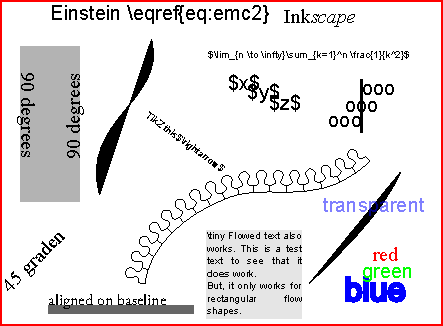
\includegraphics[width=0.5\columnwidth]{ChapterTemplate/image-normal.pdf}
      \caption[The test SVG image, as it is seen in Inkscape]
      {The test SVG image, as it is seen in Inkscape (exported to PDF
      \emph{without} \LaTeX\ option).}
      \label{fig:normal}
\end{figure}

\begin{figure}
\centering
    \includesvg[width=0.8\columnwidth]{image}
    \caption{The test image, exported to PDF \emph{with} \LaTeX\ option.}
    \label{fig:pdflatex}
\end{figure}

\begin{equation}
    \label{eq:emc2}
    E = mc^{2}
\end{equation}

\subsubsection{Automatic export}

(`write18' must be enabled, see the {\small\verb|epstopdf|} package
documentation. Add {\small\verb|-shell-escape|} to the command line when calling
{\small\verb|pdflatex|}. \textcolor{red}{And inkscape must be discoverable by the
OS}),

Whenever the SVG file is updated, it is possible to have \LaTeX\ automatically call Inkscape to export the image to PDF and \LaTeX\ again. This simplifies the workflow to
\begin{itemize}
	\item Modify the SVG image in Inkscape;
	\item Save the SVG (Ctrl+S, no need to export to PDF);
	\item Recompile \LaTeX\ document. pdf\LaTeX\ will notice the SVG file has changed, and will automatically do the export for you.
\end{itemize}

\section{Math}

The following equation uses a custom mathematical operator defined in line 88
of preamble.tex:
\begin{equation}
\begin{aligned}
            \meshgrid_{\mathbf{x}_{1},\mathbf{x}_{2}}\mathbf{x}_{1}&=
            \begin{bmatrix}a_{1} & b_{1} & c_{1}\\
            a_{1} & b_{1} & c_{1}
\end{bmatrix}\\
            \meshgrid_{\mathbf{x}_{1},\mathbf{x}_{2}}\mathbf{x}_{2}&=
            \begin{bmatrix}a_{2} & a_{2} & a_{2}\\
            b_{2} & b_{2} & b_{2}
\end{bmatrix}
\end{aligned}
\end{equation}

The following equation uses the custom ceil and floor operator defined in line 86 of the stock preamble.tex:

\begin{equation}
x = \floor*{\frac{y}{2}} + \ceil*{\frac{w}{2}}
\end{equation}


And this is an equation with multiple lines:
\begin{equation}
\begin{aligned}
&I_{0}=I^{\prime}+I^{\prime\prime}\cos(\varPsi)   \\
&I_{\pi/2}=-I^{\prime\prime}\sin(\varPsi)                \\
&I_{\pi}=I^{\prime}-I^{\prime\prime}\cos(\varPsi)   \\
&I_{3\pi/2}=I^{\prime\prime}\sin(\varPsi)
\end{aligned}
\end{equation}

And this is some random Python code:

\begin{lstlisting}[style = Python]
def Hello():
    """
      Meaningful docstring with in-depth explanation of this function
    """
    print(``Hello World !!'')

if __name__ == '__main__':
    Hello()
\end{lstlisting}
\section{Abreviations}

Use acronyms like this: \ac{ann}
% Add others as needed


%-------------------------------------------------------------------------
%	BIBLIOGRAPHY
%-------------------------------------------------------------------------
\addvspacetoc{0.5cm}
\addtotoc{Bibliography}

%\fancyhead[LO]{\textsc{Bibliography}}

 % The references are stored in the file "Bibliography.bib"
\bibliography{Bibliography}

%-------------------------------------------------------------------------
%	THESIS CONTENT - APPENDICES
%-------------------------------------------------------------------------

\appendix % Cue to tell LaTeX that the following 'chapters' are Appendices

%%% -----------  ADD APPENDIX HERE ------------------ %%%

% Appendix Template

\chapter*{Appendix Title Here} % Main appendix title

\label{AppendixX} % Change X to a consecutive letter; for referencing this appendix elsewhere, use \ref{AppendixX}

Write your Appendix content here.
%\input{Appendices/AppendixB}
%\input{Appendices/AppendixC}

\backmatter


\end{document}
